\documentclass[12pt]{article}
\usepackage{fullpage}
\usepackage{titlesec}
\usepackage{tikz}
\usepackage{amsfonts,amssymb}
\usepackage{amsmath}
\usepackage{comment}
\usepackage{multicol}
\usetikzlibrary{automata, positioning}

\input ../libraries/mac.tex
\input ../libraries/mathmac.tex

\begin{document}
\pagestyle{plain}
\titleformat{\subsection}[runin]
  {\normalfont\large\bfseries}{\thesubsection}{1em}{}

\title{Homework 4}
\author{Brooke Fugate, Michael O'Connor, Rohan Shah}
\date{}

\maketitle

\section*{Problem B1}
\subsection*{(i)}
We can prove the language $L$ is not regular by contradiction, so assume that
$L$ is regular. Thus, its complement $\overline{L}$ must also be regular.
Further, given the trivially regular language $X = \{a^+b^+\}^+$, the language
$L' = \overline{L} \cap X$ must also be regular, where
$L' = \{(a^+b^+)^n\ |\ n \text{ is prime}\}$. But we have previously
shown that a language consisting of exactly a prime number of concatenation
of words in $\Sigma^*$ is not regular which is a contradiction thus, $L$ is not
regular.
\medskip
\newline
To prove that the pumping lemma holds for the language $L$ we must show that
there exists some $m \ge 1$ such that for all $w \in \Sigma^*$, if $w \in L$
and $|w| \ge m$, there exists $u,x,v \in \Sigma^*$ such that $w = uxv$,
$x \neq \epsilon$, $|ux| \le m$, and $ux^iv \in L$ for all $i \ge 0$. Let
$m = 9$ and consider a $w \in L$ where $|w| \ge m$. Then there exists a
prefix of $w$ of length $m$, i.e. there exists some $w_p,w_s \in \Sigma^*$
such that $w = w_pw_s$ and $|w_p| = m$. If we do case analysis on
$w_p$ we can see that it can take one of two different forms. The first is the
case where there exists a substring $s \in \Sigma^*$ of $w_p$ such that
$s = a^i$ or $s = b^i$ where $i \ge 2$. The second case is the alternate where
there does not exist such a substring $s$ in $w_p$, i.e. $w_p$ consists solely
of substrings of the form $ab$. Both these cases are due to the fact that
$w \in L$. We will show that the pumping lemma holds in both these cases.
\medskip
\newline
Consider the first case. Let $w_p = uxv'$ such that $u$ is the prefix of
$w_p$ up till the occurence of the first substring of the form $a^i$ or $b^i$
where $i \ge 2$. Then let $x = a$ or $x = b$ respectively. Finally let $v$ be
the remaining suffix of our original word $w$ (by our previous definitions this
means $v = (a | b)^jv'w_s)$ but this is not important to the proof).
By definition $w = uxv$ and $x \neq \epsilon$. Further $|ux| \le m$ since both
$ux$ is a prefix of $w_p$ which we defined such that $|w_p| = m$. Finally since
$x$ is the single character $a$ or $b$ of a substring of $w$ where there are
more than one $a$'s or $b$'s respecitvely, pumping down once or pumping up
infinitely does not change the value of $n$ in the definition of $L$ meaning
that it remains non prime, nor does it change the form of $w$ meaning $w$
maintains the form $w = x_1y_1 \cdots x_ny_n$, therefore $ux^iv \in L$ for all
$i \ge 0$ and thus the pumping lemma holds for words $w$ in this case.
\medskip
\newline
Now consider the second case. We know that $w = ababababaz$ for some
$z \in \Sigma^*$ and thus that $w_p = ababababa$. Since all we know about $n$ is
that it's not prime, it could be either odd or even. So consider first when $n$
is odd. Let $u = a$, $x = b$, and $v$ be the rest of $w$ i.e. $v = abababaz$. By
construction $w = uxv$, $x \neq \epsilon$, and $|ux| = 2 \le m = 9$. Pumping
down, meaning removing $x$, maintains the form of $w$ but decreases $n$ by 1.
But since $n$ is odd this makes $n$ even which is not prime. Pumping up does
not change $n$ and thus $n$ remains non prime and of the required form
thus the pumping lemma holds when $n$ is odd. Now consider the case when $n$ is
even. Let $u = \epsilon$, $x = abab$, and $v$ be the rest of $w$ i.e.
$v = ababaz$. By construction $w = uxv$, $x \neq \epsilon$, and
$|ux| = 4 \le m = 9$. Pumping down, meaning removing $x$, does not change the
form of $w$ but does decrease $n$ by 2. But since $n$ is even, $n$ remains even
and thus $n$ is not prime. Pumping up also lets $n$ remain even and of the
required form. Thus, the pumping lemma also holds when $n$ is even.
\medskip
\newline
Therefore the pumping lemma holds in all cases of $w \in L$ where $|w| \ge m = 9$,
thus the pumping lemma holds for the language $L$ even though $L$ is not regular.

\subsection*{(ii)}
To prove that this pumping lemma holds for any regular language $L$ we must show
that there exists some $m \ge 1$ such that for all $y \in \Sigma^*$,
if $y \in L$ and $|y| = m$, there exists $u,x,v \in \Sigma^*$ such that
$y = uxv$, $x \neq \epsilon$, and for all $z \in \Sigma^*$,
$yz \in L \iff ux^ivz \in L$ for all $i \ge 0$. Since $L$ is a regular language
it has a finite, positive, non-zero number of Myhill-Nerode equivalence classes.
Let $m$ be equal to this number. Now consider any word $y \in L$ where $|y| = m$.
There are $m+1$ prefixes of the word $y$ (including $\epsilon$ and $y$). Since
there are only $m$ equivalence classes for the language $L$ there must exists
two prefixes of $y$, namely $p_1,p_2 \in \Sigma^*$ such that $p_1 \simeq_D p_2$
and $|p_1| > |p_2|$. Therefore it follows that $p_2$ is also a prefix of $p_1$
so $p_1 = p_2x'$ for some $x' \in \Sigma^*$ where $|x'| \neq 0$ which implies
$x' \neq \epsilon$. Let $x=x'$, $u=p_2$, and $v$ be the suffix of $y$
such that $y=p_1v$. Thus we have $y = uxv$ and $x \neq \epsilon$ by construction.
We also have $u \simeq_D ux$ by substitution. Now we just need to prove that
$yz \in L \iff ux^ivz \in L$ for all $i \ge 0$.
Since $y = uxv$ this is equivalent to proving $uxvz \in L \iff ux_ivz \in L$.
But we can show something stronger than this, namely that $uxvz \simeq_D ux^ivz$
which directly implies that $uxvz \in L \iff ux^ivz \in L$ by the way in which
Myhill-Nerode string equivalence is defined. Further, we can prove
$uxvz \simeq_D ux^ivz$ for all $z \in \Sigma^*$ by proving $uxv \simeq_D ux^iv$
for all $i \ge 0$ and applying the right-invariance property of Myhill-Nerode
equivalence. Given $u \simeq ux$ from above and using right-invariance we have
$ux \simeq_D ux^2$. By transitivity and induction we have $ux \simeq_D ux^i$
for all $x \ge 0$. By right-invariance again we have $uxv \simeq_D ux^iv$ which
is what we wanted to prove therefore the pumping lemma holds for all regular
languages $L$.

\subsection*{(iii)} The equivalence relation $\rho_L$ is defined such that
for any two strings $u, v \in \Sigma^*$
$$ u\ \rho_L\ v \iff \forall z \in \Sigma^*,\ uz \in L \iff vz \in L$$
Further, $L$ is the union of the equivalence classes of strings in $L$ i.e.
$$L = \bigcup _{u\in L} [u]_{\rho_L}$$
Since we are given that $L$ satisfies the modified pumping lemma we have the
following condition
$$y\ \rho_L\ ux^iv$$
Thus, to prove that the language $L$ is regular we just need to prove that the
equivalence relation $\rho_L$ has a finite index.
\newline
\textbf{Claim: } For any string $w \in \Sigma^*$ such that $|w| \ge m$ there
exists a string $w' \in \Sigma^*$ such that $|w'| < m$ and $w\ \rho_L\ w'$.
\newline
\textbf{Proof: } Let $w \in \Sigma^*$ such that $|w| \ge m$. Then there is a
decomposition of $w$ into a prefix and suffix such that $w = w_pw_s$ such that
$|w_p| = m$. Since we assume the pumping lemma holds we have $w_p = uxv$ such
that $x \neq \epsilon$ and
$\forall z \in \Sigma^*,\ w_pz \in L \iff ux^ivz \in L,\ \forall i \ge 0$.
Let $z = w_sz'$. Therefore we have
$$ w_pz \in L \iff ux^ivz \in L$$
$$\implies w_pw_sz' \in L \iff ux^ivw_sz' \in L$$
$$\implies wz' \in L \iff uvw_sz' \in L\ (i = 0 \therefore x = \epsilon)$$
$$\equiv w\ \rho_L\ uvw_s$$
Let $w' = uvw_s$ then we have $w\ \rho_L w'$ such that $|w| > |w'|$ since
$|w| = |uxvw_s| = |uvw_s|+|x| = |w'| +|x|$ where $|x| > 0$ since
$x \neq \epsilon$. If $|w'| \ge m$ we can repeat this process until we reach a
$w'$ such that $w'$ such that $|w'| < m$ and $w'\ \rho_L w$.
Since we have proven that for any string $w \in \Sigma^*$ such that $|w| \ge m$
there exists a string $w' \in \Sigma^*$ such that $|w'| < m$ and $w\ \rho_L\ w'$
and since $m$ is a finite index there exist only a finite number of words $w'$
such that $|w'| < m$, there are a finite number of $\rho_L$ equivalence classes.
Thus if a language $L$ holds for the modified pumping lemma then it is regular.

\subsection*{(iv)}
\subsection*{(v)}

\newpage
\section*{Problem B3}
\textbf{Claim:} There are infinitely many primes of the form $4n+3$.
\newline
\textbf{Proof:} Say we already have $n+1$ of these primes, denoted by
$$3, p_1, p_2, \cdots, p_n,$$
where $p_i > 3$. Consider the number
$$m = 4p_1p_2 \cdots p_n + 3$$
and its prime factorization
$$m=q_1 \cdots q_k.$$
First we can prove that $q_j > 3$ for $j = 1,...,k$. Since any number of the
form $4n+3$ is odd $2$ can not be a prime factor of it therefore $q_j \neq 2$.
We can finish the proof by
contradiction, so assume there exists some $q_j = 3$. Since $q_j$ is a prime
factor of $m$ we know that
$$m\ \mod\ q_j = 0 \implies (4p_1p_2 \cdots p_n + 3)\ \mod\ 3 = 0
\implies (4p_1p_2 \cdots p_n)\ \mod\ 3 = 0$$
which is a contradiction because
$$4\ \mod\ 3 \neq 0,p_1\ \mod\ 3 \neq 0,...,p_n\ \mod\ 3 \neq 0.$$
Therefore $q_j > 3$. Now we can prove that for all $p_i$ and $ q_j$,
$p_i \neq q_j$ by contradiction so assume there exists some $p_i$ and $q_j$ such
that $p_i = q_j$. Since $q_j$ is a prime factor of m and $q_j = p_i$ it must be
true that
$$(4p_1p_2 \cdots p_n + 3)\ \mod\ p_i = 0.$$
And it is true that
$$(4p_1p_2 \cdots p_n)\ \mod\ p_i = 0.$$
Therefore
$$(4p_1p_2 \cdots p_n + 3)\ \mod\ p_i = 0 \iff 3\ \mod\ p_i = 0$$
which is equivalent to
$$3\ \mod\ q_j = 0$$
which is a contradiction since $q_j > 3$, therefore $p_i \neq q_j$ for all $p_i$
and $q_j$. Finally we can prove that there exists a $q_j$ of the form $4n+3$.
Observe that all odd numbers are either of the form $4n+1$ or $4n+3$. Also
observe that given two numbers of the form $4n+1$, say $x = 4m+1$ and
$y = 4n+1$ then $xy = 4(4mn + m + n) + 1$ which is again of the form $4n+1$.
We can proceed by contradiction so assume there are no $q_j$ of the form
$4n+3$ therefore all $q_j$ must be of the form $4n+1$ which implies that
$q_1q_2\cdots q_n$ is of the form $4n+1$ which is a contradiction since $m$ is
of the form $4n+3$ therefore there must exists a $q_j$ of the form $4n+3$.
Since, there exists a $q_j$ of the form $4n+3$ that is greater than $3$ and not
equal to any of the first $(n+1)$ $p_i$ of the form $4n+3$ and since $q_j$ is a
prime factor of $m$, there exists a prime number of the form $4n+3$ greater than
all previous primes of the form $4n+3$ so by induction there are an infinite
number of primes of the form $4n+3$.
\medskip
\newline
Now that we have proven that there are infinitely many primes of the form $4n+3$
we know that the language $L$ is infinte. We can prove that $L$ is not regular
by contradiction using Myhill-Nerode equivalence. Assume $L$ is regular. Then
there exists a finite number of Myhill-Nerode equivalence classes. Since $L$ is
infinite there exists two words $w,w' \in L$ where $w = a^i$ and $w' = a^j$ such
that $i$ and $j$ are prime numbers of the form $4n+3$, $i <j$, and
$a^i \simeq_D a^j$.
Since $i < j$ there exists
some $r > 0$ such that $i + r  = j$. Therefore $a^i \simeq a^{i+r}$.
By right-invariance, $a^i \simeq a^{i+r} \implies a^{i}z \simeq a^{i+r}z,
\ \forall z \in \Sigma^*$. Let $z = a^r \in \Sigma^*$ then
$a^{i}a^{r} \simeq a^{i+r}a^{r} \equiv
a^{i+r} \simeq a^{i+2r}$. By transitivity, $a^i \simeq a^{i+2r}$ and by
induction, $a^i \simeq a^{i + kr},\ \forall k \ge 0$. Let $k = i$, then
$a^i \simeq a^{i+ir} = a^{i(1+r)}$. Therefore, $a^i \simeq a^{ix}$.
Since $i < ix$, $x \ge 2$, therefore $ix$ is not prime. So
$a^i \simeq a^{ix}$ but $a^i \in L$ and $a^{ix} \notin L$ which is a
contradiction thus $L$ is not regular.

\section*{Problem B4}
\textbf{Claim: } For every $w \in \Sigma^*$ and for every state, $T\subseteq Q$,
of $D^R$,
$$\delta_R^*(T, w) = \{q\in Q \mid \delta^*(q, w^R) \in T\}$$
where $\delta_R$ is the transition function of $D^R$.
\newline
\textbf{Proof: } By induction on $|w|$, the length of $w$.
\newline
Base Case: $|w|= 0$ therefore $w = \epsilon$.
$$\delta_R^*(T, \epsilon) = \{q\in Q \mid \delta^*(q, \epsilon) \in T\}$$
$$T = \{q \in Q\ |\ q \in T\}$$
$$T = T$$
\newline
Inductive Case: $|w| = n+1$ therefore $w = ua$ such that $a \in \Sigma$,
$u \in \Sigma^*$, and $|u| = n$.
Induction Hypothesis: $\delta_R^*(T, u) = \{q\in Q \mid \delta^*(q, u^R) \in T\}$
$$\delta_R^*(T, w) = \delta_R^*(T, ua) = \delta_R(\delta_R^*(T,u),a)$$
$$= \{q \in Q \mid \delta(q,a) \in \delta_R^*(T,u)\} =
\{q\in Q \mid \delta^*(q, au^R) \in T\}$$
$$= \{q\in Q \mid \delta^*(q, (ua)^R) \in T\} =
\{q\in Q \mid \delta^*(q, w^R) \in T\}$$
\medskip
\newline
\textbf{Claim: } $D^R$ is a minimal DFA for the language $L(D^R)$.
\newline
\textbf{Proof: } Let $D^R = \{Q_R, \Sigma, \delta_R, S_0, F_R\}$. We can prove
that $D^R$ is minimal by proving that no two states $S, T \in Q_R$ are
equivalent i.e. $S \not\equiv T$. In $D^R$, $S \equiv T$ iff
$$ \forall w \in \Sigma^*,\ \delta_R^*(S,w^R) \in F_R \iff
\delta_R^*(T,w^R) \in F_R$$
By construction of $D^R$ we have
$$ \forall w \in \Sigma^*,\ \forall S \in Q_R,\ \delta_R^*(S, w^R) \in F_R \iff
q_0 \in \delta_R^*(S, w^R)$$
Therefore, we can use substitution to come up with an alternate definition for
state equivalence, i.e. $S \equiv T$ iff
$$ \forall w \in \Sigma^*,\ q_0 \in \delta_R^*(S, w^R) \iff
q_0 \in \delta_R^*(T, w^R)$$
By construction of $D^R$ we also have the property that
$$ \forall w \in \Sigma^*,\ S \in Q_R,\ q_0 \in \delta_R^*(S, w^R) \iff
\delta^*(q_0, w) \in S$$
Therefore, we can use substitution again to come up with another statement
of state equivalence for $D^R$, i.e. $ S \equiv T$ iff
$$ \forall w \in \Sigma^*,\ \delta^*(q_0, w) \in S \iff \delta^*(q_0, w) \in T$$
But since $D$ is deterministic there exists a single state $p \in Q$ such
that $\delta^*(q_0, w) = p$. Which gives us another definition for state
equivalence i.e. $S \equiv T$ iff
$$ \forall w \in \Sigma^*,\ \exists p \in Q,\ \delta^*(q_o,w) = p \implies
p \in S \iff p \in T$$
We can now show that $S \not\equiv T$ for all $S,T \in Q_R$ by contradiction.
So assume there exist two states $S,T \in Q_R$ such that $S \equiv T$ therefore
for all $w \in \Sigma^*$, there exists a state $p \in Q$ such that
$\delta^*(q_0,w) = p$ and $p \in S \iff p \in T$. But by construction of $D^R$
we have that
$$\forall w \in \Sigma^*,\ \exists p \in Q,\ \delta^*(q_0, w) = p \implies
\exists S \in Q_R,\ p \in S,\ \delta_R^*(S_0, w^R) = S$$
Therefore our above statement can be rewritten using substitution to state that
a final definition of state equivalence for $D^R$:
$$ S \equiv T \iff \forall w \in \Sigma^*,
\delta_R^*(S_0, w^R) = S \iff \delta_R^*(S_0, w^R) = T$$
which is a contradiction since $D^R$, and thus its extended transition function
$\delta_R^*$, are deterministic. Therefore $D^R$ is a minimal DFA.
\medskip
\newline
We can now prove that $D^{RR}$ is a minimal DFA for L. First we prove
that $D^{RR}$ is a DFA that defines the language $D$ i.e. $L(D^{RR}) = L$.
$$L(D^{RR}) = L(D^R)^R = L(D)^{RR} = L^{RR} = (L^R)^R = L$$
Finally we can prove that $D^{RR}$ is a minimal DFA for the language $L(D^{RR})$
given a DFA $D$ for the language $L$ from which we construct it. We can take
$D$ and construct the DFA $D^R$ for the language $L^R$, which we have proven is
minimal. We can now take the DFA $D^R$ and construct the DFA $D^{RR}$ for
the language $L(D^{RR})$, which by the same proof is minimal.

\newpage
\section*{Problem B5}
\subsection*{(a)}
Let $M = (K, \Sigma, \Delta, \lambda, q_0, F)$ be an $a$-transducer where
$K = F = \{q_0\}$, $\Sigma = \Delta = \{a,b\}$ and we can define $\lambda$
by induction over the words $u\in \Sigma^*$ and $v \in \Delta^*$ such that
$(q_0, \epsilon, \epsilon, q_0) \in \lambda$ is the base case and by induction
if $(q_0, u, v, q_0) \in \lambda$ then $(q_0,au,bv,q_0), (q_0,bu,av,q_0) \in
\lambda$. A figure that illustrates the $a$-transducer $M$ is:
\begin{center}
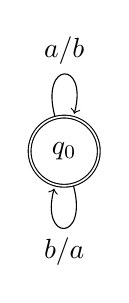
\begin{tikzpicture}[shorten >=1pt, node distance=2.5cm, on grid, auto]
  \node[state, accepting] (q0) {$q_0$};
  \path[->]
(q0) edge [loop above] node {$a/b$} (q0)
(q0) edge [loop below] node {$b/a$} (q0)
  ;
\end{tikzpicture}
\end{center}

\subsection*{(b)}
To prove that the language $R$ is regular we will construct an NFA $N$ using
the given $a$-transducer $M = (K, \Sigma, \Delta, \lambda, q_0, F)$ and alphabet
$T = \{[p,u,v,q] \mid (p,u,v,q) \in \lambda\}$ and prove that $L(N) = R$ thereby
proving $R$ is regular by NFA construction. Let $N = (K, T, \delta, q_0, F)$
where $\delta$ is defined such that
$$\forall p \in K,\ \delta(p, [p,u,v,q]) = q \iff [p,u,v,q] \in \lambda$$
We also define the language $R'$ such that $R \subseteq R'$ where
$$R' = \{[q_o, u_1,v_1,q_1] \cdots [q_{m-1},u_m,v_m,q_m] \mid
[q_{i-1},u_i,v_i,q_i] \in T, 1 \le i \le m, m \ge 1\} \cup \{\epsilon\}$$
and the function $\sigma : T^* \rightarrow K$ such that
$$\sigma(\epsilon) = q_0$$
$$\forall a \in T^* \text{ where }
a = a'[p,u,v,q],\ \sigma(a) = \sigma(a'[p,u,v,q]) = q$$
\textbf{Claim: } $\forall a \in T^*,\ \delta^*(q_0, a) = q \iff a \in R'
\text{ and } \sigma(a) = q$
\newline
\textbf{Proof: } By induction on the length of $a$.
\newline
Base Case: $|a| = 0$ therefore $a = \epsilon$.
$$\delta^*(q_0, \epsilon) = q_0 = \sigma(\epsilon) \text{ and }\epsilon \in R'$$
Inductive Case: $|a| = n+1$ therefore $a = a'[p,u,v,q]$ such that $a,a' \in T^*$
and $|a'| = n$.
Induction Hypothesis: $\delta^*(q_0, a') = p \implies a' \in R' \text{ and }
\sigma(a') = p$
$$ \delta^*(q_0, a) = \delta^*(q_0, a'[p,u,v,q]) =
\delta(\delta^*(q_0, a') ,[p,u,v,q]) = \delta(p, [p,u,v,q) = q$$
$$\sigma(a) = \sigma(a'[p,u,v,q]) = q$$
$$a' \in R \implies a'b \in R,\ \forall b \in T \implies a'[p,u,v,q] \in R
\implies a \in R$$
Since we know that $R \subseteq R'$ we can use the above claim to rewrite the
language $R$ as $$R = \{a \in R' \mid \sigma(a) \in F\}$$
We can now finish our proof by proving that $L(N) = R$.
$$L(N) = \{a \in T^* \mid \delta^*(q_0, a) \in F\}$$
$$\delta^*(q_0, a) \in F \iff \sigma(a) \in F \text{ and } a \in R'
\text{ (by the above claim)}$$
$$L(N) = \{a \in R' \mid \sigma(a) \in F\} = R$$
Therefore, since the NFA $N$ defines the language, $R$ is regular.

\subsection*{(c)}
Given the homomorphism $f : T^* \rightarrow \Sigma^*$ we can define the inverse
image of the language $L \subseteq \Sigma^*$ as
$$f^{-1}(L) = \{a \in T^* \mid f(a) \in L)$$
And we know that $a\in T^*$ implies that $a = a_1a_2 \cdots a_n$ such that
$a_i \in T$, $n \ge 0$, and $a_i = [p_i, u_i, v_i, q_i]$.
We also know that $f([p,u,v,q]) = u$ by the definition of our homomorphism so
$$f(a) = f(a_1a_2\cdots a_n) = f(a_1)f(a_2)\cdots f(a_n) = u_1u_2\cdots u_n$$
Therefore we can rewrite the inverse image of $L$ as
$$f^{-1}(L) =
\{[p_1,u_1,v_1,q_1][p_2,u_2,v_2,q_2]\cdots [p_n,u_n,v_n,q_n] \in T^*$$
$$\mid [p_i,u_i,v_i,q_i] \in T,\ u_1u_2\cdots u_n \in L,\ n \ge 1\} \cup
\{\epsilon \mid \epsilon \in L\}$$
and by definition we have
$$ R = \{[q_0, u_1, v_1, q_1][q_1, u_2, v_2, q_2]\cdots
[q_{n-2}, u_{n-1}, v_{n-1}, q_{n-1}][q_{n-1}, u_n, v_n, q_n]$$
$$\mid  [q_{i-1}, u_i, v_i, q_i]\in T,\, q_n\in F,\, n\geq 1\}
\cup \{\epsilon\ |\ q_0\in F\}$$
thus we have
$$f^{-1}(L)\cap R  = \{[q_0, u_1, v_1, q_1][q_1, u_2, v_2, q_2]\cdots
[q_{n-2}, u_{n-1}, v_{n-1}, q_{n-1}][q_{n-1}, u_n, v_n, q_n]$$
$$ \mid  [q_{i-1}, u_i, v_i, q_i]\in T,\, u_1u_2\cdots u_n\in L,\,
q_n\in F,\, n\geq 1\}\cup \{\epsilon\ |\ q_0\in F,\, \epsilon\in L\}$$
which is what we are trying to prove.

\subsection*{(d)}
Given the homomorpism $g : T^* \rightarrow \Delta$ we can define the image of
the language $f^{-1}(L)\cap R\subseteq T^*$ as
$$g(f^{-1}(L)\cap R) = \{g(a) \mid a \in f^{-1}(L)\cap R\}$$
and we know that $a \in f^{-1}(L)\cap R$ implies that $$a =
[q_0, u_1, v_1, q_1][q_1, u_2, v_2, q_2]\cdots
[q_{n-2}, u_{n-1}, v_{n-1}, q_{n-1}][q_{n-1}, u_n, v_n, q_n]$$ such that
$[q_{i-1}, u_i, v_i, q_i]\in T$, $u_1u_2\cdots u_n\in L$, $q_n\in F$ and
$n\geq 1$. And by the construction of $T$ we have that if $[p,u,v,q] \in T$
then $(p,u,v,q) \in \lambda$. By the definition of an $a$-transducer we have
that if $(p,u,v,q) \in \lambda$ then $(p, u\alpha, \beta) \vdash_M (q,a,\beta v)$
and by transitive and reflexive closure
$(p,w, \epsilon) \vdash_M^* (q,\epsilon,y)$ for some $w \in \Sigma^*$ and
$y \in \Delta^*$. Therefore $a \in f^{-1}(L)\cap R$ implies
$(q_0,w,\epsilon) \vdash_M^* (q_n, \epsilon, y)$ such that $q_n \in F$.
And, since $g([p,u,v,q]) = v$ we have $g(a) = v_1v_2\cdots v_n \in \Delta^*$ by
a similar proof to the one briefly described for $f(a)$ in the previous part.
So we can rewrite the image of $f^{-1}(L)\cap R$ as
$$g(f^{-1}(L)\cap R) = \bigcup _{w\in L} \{y \in \Delta^*
\mid (q_0, w, \epsilon) \vdash_M^* (q_n, \epsilon, y),\ q_n \in F\} =
\bigcup _{w\in L} M(w) = M(L)$$
which is what we wanted to prove. We can also show that $\s{L}$ is closed under
$a$-transduction. We have $f^{-1}(L) \in \s{L}$ by the fact that $\s{L}$ is
closed under inverse homomorphic images. Since we proved that $R$ is regular we
also have that $f^{-1}(L) \cap R \in \s{L}$ by the fact that $\s{L}$ is closed
under intersection with regular languages. Finally we have that
$g(f^{-1}(L) \cap R) \in \s{L}$ by the fact that $\s{L}$ is closed under
homomorphic images. And we just proved that $g(f^{-1}(L) \cap R) = M(L)$ so we
have $M(L) \in \s{L}$ which means $\s{L}$ is closed under $a$-transduction.
Finally we can prove that if $L$ is regular then $M(L)$ regular. Since $L$ is
regular, and the regular languages are closed under intersection, homomorphism,
and inverse homomorphism, we know that $g(f^{-1}(L) \cap R) = M(L)$ is regular.

\subsection*{(e)}
We can define an $a$-transducer, $M_2 = (K, \Delta,\Sigma,\lambda_2,q_0, F)$
such that $(q,v,u,p) \in \lambda_2 \iff (p,u,v,q) \in \lambda$. It is clear then
that $L(M_2) = M^{-1}(L')$ where
$$M^{-1}(L') = \bigcup _{y\in L'} M^{-1}(y)
= \bigcup _{y\in L} \{w \in \Sigma^* \mid y \in M(w)\}$$
$$ = \bigcup _{y\in L'} \{w \in \Sigma^*
\mid y \in \{y \in \Delta^*
\mid (q_0, w, \epsilon) \vdash_M^* (f, \epsilon, y),\ f \in F\}\}$$
$$= \{w \in \Sigma^* \mid (q_0, w, \epsilon) \vdash_M^* (f, \epsilon, y)
,\ f\in F, y\in \Delta^*\}$$
Therefore, since the language $M^{-1}(L')$
is defined by an $a$-transducer and we have already proven that regular languages
are closed under $a$-transduction, if $L'$ is regular then $M^{-1}(L')$ is also
regular.

\newpage
\section*{Problem B6}
\subsection*{(1)}
\begin{center}
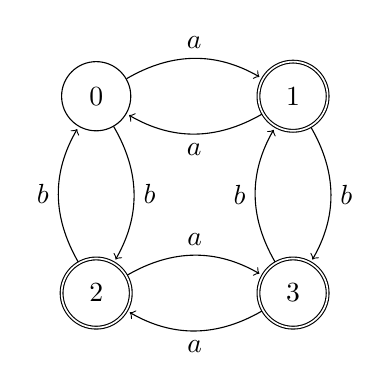
\begin{tikzpicture}[shorten >=1pt, node distance=2.5cm, on grid, auto]
  \node[state] (q0) {0};
  \node[state, accepting] (q1) [right=of q0] {1};
  \node[state, accepting] (q2) [below=of q0] {2};
  \node[state, accepting] (q3) [right =of q2] {3};
  \path[->]
(q0) edge [bend left] node {$a$} (q1)
(q0) edge [bend left] node {$b$} (q2)
(q1) edge [bend left] node {$a$} (q0)
(q1) edge [bend left] node {$b$} (q3)
(q2) edge [bend left] node {$a$} (q3)
(q2) edge [bend left] node {$b$} (q0)
(q3) edge [bend left] node {$a$} (q2)
(q3) edge [bend left] node {$b$} (q1)
  ;
\end{tikzpicture}
\end{center}

\subsection*{(2)}
$(\epsilon +(a+b)(bb+(a+b)(a+b))^*(\epsilon +a+b))+
((\epsilon +a+b)+(a+b)(bb+(a+b)(a+b))^*(ba+(a+b)(a+b)))
((aa+(a+b)(a+b)+(ab+(a+b)(a+b))(bb+(a+b)(a+b))^*(ba+(a+b)(a+b)))^*
((a+b)+(ab+(a+b)(a+b))(bb+(a+b)(a+b))^*(\epsilon+a+b))$

\subsubsection*{Node Elimination Steps:}
\textbf{Initial Edges}
\begin{multicols}{4}
\noindent
$(0,1) = a$\\
$(0,2) = b$\\
\columnbreak
\break
$(1,0) = a$\\
$(1,3) = b$\\
\columnbreak
\break
$(2,0) = b$\\
$(2,3) = a$\\
\columnbreak
\break
$(3,1) = b$\\
$(3,2) = a$\\
\end{multicols}

\noindent\textbf{After Preprocessing}
\begin{multicols}{5}
\noindent
$(s,0) = \epsilon$\\
$(s,1) = \emptyset$\\
$(s,2) = \emptyset$\\
$(s,3) = \emptyset$\\
$(s,t) = \emptyset$\\
\columnbreak
\break
$(0,0) = \emptyset$\\
$(0,1) = a$\\
$(0,2) = b$\\
$(0,3) = \emptyset$\\
$(0,t) = \emptyset$\\
\columnbreak
\break
$(1,0) = a$\\
$(1,1) = \emptyset$\\
$(1,2) = \emptyset$\\
$(1,3) = b$\\
$(1,t) = \epsilon$\\
\columnbreak
\break
$(2,0) = b$\\
$(2,1) = \emptyset$\\
$(2,2) = \emptyset$\\
$(2,3) = a$\\
$(2,t) = \epsilon$\\
\columnbreak
\break
$(3,0) = \emptyset$\\
$(3,1) = b$\\
$(3,2) = a$\\
$(3,3) = \emptyset$\\
$(3,t) = \epsilon$\\
\end{multicols}

\noindent\textbf{After Eliminating Node 1}
\begin{multicols}{4}
\noindent
$(s,0) = \epsilon + a$\\
$(s,2) = \emptyset$\\
$(s,3) = \emptyset + b$\\
$(s,t) = \epsilon$\\
\columnbreak
\break
$(0,0) = aa$\\
$(0,2) = b+a$\\
$(0,3) = ab$\\
$(0,t) = a$\\
\columnbreak
\break
$(2,0) = b+a$\\
$(2,2) = \emptyset$\\
$(2,3) = a+b$\\
$(2,t) = \epsilon$\\
\columnbreak
\break
$(3,0) = ba$\\
$(3,2) = a+b$\\
$(3,3) = b$\\
$(3,t) = \epsilon+b$\\
\end{multicols}

\noindent\textbf{After Eliminating Node 2}
\begin{multicols}{3}
\noindent
$(s,0) = (\epsilon + a+b)$\\
$(s,3) = (a+b)$\\
$(s,t) = \epsilon$\\
\columnbreak
\break
$(0,0) = (aa+(b+a)(b+a))$\\
$(0,3) = (ab+(b+a)(a+b))$\\
$(0,t) = (a+b)$\\
\columnbreak
\break
$(3,0) = (ba+(a+b)(b+a))$\\
$(3,3) = (b+(a+b)(a+b))$\\
$(3,t) = ((\epsilon+b)+(a+b)(\epsilon + b))$\\
\end{multicols}

\noindent\textbf{After Eliminating Node 3}\\
$(s,0) = ((\epsilon + a+b) + (a+b)(b+(a+b)(a+b))^*(ba+(a+b)(b+a)))$\\
$(s,t) = (\epsilon + (a+b)(b+(a+b)(a+b))^*((\epsilon+b)+(a+b)(\epsilon + b)))$\\
$(0,0) = ((aa+(b+a)(b+a)) + (ab+(b+a)(a+b))(b+(a+b)(a+b))^*(ba+(a+b)(b+a)))$\\
$(0,t) = ((a+b) + (ab+(b+a)(a+b))(b+(a+b)(a+b))^*((\epsilon+b)+(a+b)(\epsilon + b)))$\\

\noindent\textbf{After Eliminating Node 0}\\
$(s,t) = (\epsilon + (a+b)(b+(a+b)(a+b))^*((\epsilon+b)+(a+b)(\epsilon + b))) +
((\epsilon + a+b) + (a+b)(b+(a+b)(a+b))^*(ba+(a+b)(b+a)))
((aa+(b+a)(b+a)) + (ab+(b+a)(a+b))(b+(a+b)(a+b))^*(ba+(a+b)(b+a)))^*
((a+b) + (ab+(b+a)(a+b))(b+(a+b)(a+b))^*((\epsilon+b)+(a+b)(\epsilon + b)))
$\\

\section*{Problem B7}
\subsection*{a} S is the starting symbol. \newline
$S \rightarrow c$ \newline
$S \rightarrow aSa$ \newline
$S \rightarrow bSb$ \newline
The smallest possible string is c which is given by the first production. We can build from the beginning and end of the string simultaneously with the other two productions to ensure that the string following the c is the reverse of the string before the c.
\subsection*{b} S is the starting symbol. \newline
$S \rightarrow T$ \newline
$T \rightarrow aTBb$ \newline
$B \rightarrow b$ \newline
$B \rightarrow \epsilon$ \newline
$T \rightarrow ab$ \newline
$T \rightarrow abb$ \newline
The smallest possible strings are ab/abb which is given by replacing S with T and T with ab or abb. We build up the string with by replacting T with aTBb. That guarantees that $n \ge m$vand since B can either be b or $\epsilon$ $n \le 2m$\newline

For $K \ge 2$, same as above, except with $T \rightarrow aTBb$ changed to $T \rightarrow aTB_1B_2...B_Kb$, where the productions for $B_i$ are $B_i \rightarrow b$ and $B_i \rightarrow \epsilon$ and we have the productions $T \rightarrow abb, T \rightarrow abbb ... T \rightarrow abbb...b$ with the number of $b$'s in the last production equal to the value of K. \newline
The smallest possible string is ab which is given by replacing S with T and T with ab. We build up the string with by replacting T with aTBb.  That guarantees that $n > m$ and since any $B_j \mid 1 \le j \le k$ can either be b or $\epsilon$ $n \le km$

\subsection*{c} S is the starting symbol. \newline
$S \rightarrow S_1$ \newline
$S \rightarrow S_2$ \newline
$S_1 \rightarrow aCb$ \newline
$C \rightarrow aCb$ \newline
$C \rightarrow \epsilon $ \newline
$S_2 \rightarrow aBbb$ \newline
$B \rightarrow aBbb$ \newline
$B \rightarrow \epsilon $ \newline
We create the union of the two languages using the productions $S \rightarrow S_1$ and
$S \rightarrow S_2$. The non-terminal $S_1$ is then the starting symbol for the language $\{a^{n}b^{n}\mid n \geq 1\}$, which has a smallest string of $ab$ by the production $S_1 \rightarrow aCb$ and can grow only with the production $C \rightarrow aCb$ when an $a$ and $b$ are added at the same time. The non-terminal $S_1$ is then the starting symbol for the language $\{a^{n}b^{2n}\mid n \geq 1\}$, which has a smallest string of $abb$ by the production $S_2 \rightarrow aBbb$ and can grow only by the production $B \rightarrow aBbb$ when an $a$ and two $b$'s are added at the same time.

\subsection*{d} S is the starting symbol. \newline
$S \rightarrow S_1$ \newline
$S \rightarrow S_2$ \newline
$S_1 \rightarrow aAaBb$ \newline
$A \rightarrow aAa$ \newline
$A \rightarrow Bb$ \newline
$B \rightarrow Bb$ \newline
$B \rightarrow \epsilon $ \newline
$S_2 \rightarrow aAbbbbBbbbb$ \newline
$A \rightarrow aA$ \newline
$A \rightarrow \epsilon$ \newline
$B \rightarrow bbbbaBbbbb$ \newline
$B \rightarrow a $ \newline
$S_1$ produces the language $a^mb^na^mb^p$, the smallest string S1 can produce is abab, by producing aAaBb from $S_1$ then producing Bb from A and then $\epsilon$ from B and then again producing $\epsilon$ from the remaining B.  Instead of directly producing a single b from A we could instead produce more aAa constructions making m arbritrarily large, then finally producing an arbritary amount of b by producing Bb from A and then more Bb from B.  We can do the same for the last B to get another arbrirtrary amount of b, having $m, n, \text{ and } p \ge 1$.\newline $S_2$ produces the language $a^mb^{4n}a^pb^{4n}$, the smallest string that $S_2$ produces is abbbbabbbb which is produced by replacing A with $\epsilon$ and B with a.  We can then create an arbitrary $a^m$ by producing aA from A, we also can produce an arbritrary $a^p$ by producing bbbbaBbbbb from B, which will also produce an arbritrary $b^{4n}$.\newline S can go to either $S_1$ or $S_2$ so the language is $a^mb^na^mb^p \cup a^mb^{4n}a^pb^{4n}$.

\subsection*{e} S is the starting symbol. \newline
$S \rightarrow C$ \newline
$C \rightarrow ACB$ \newline
$A \rightarrow aa$ \newline
$A \rightarrow ab$ \newline
$A \rightarrow ba$ \newline
$A \rightarrow bb$ \newline
$B \rightarrow a$ \newline
$B \rightarrow b$ \newline
$C \rightarrow \epsilon$ \newline
The smallest string that S creates is $xy \mid x = \text{ combination of 2 }a/b \text{ characters}, y =  a \text{ or } b$, so $|x| = 2|y|$, we get this by producing ACB from C and then a final production from A and B.  We could keep producing ACB from C to get an arbritarily large $|y|$ and therefore $|x| = 2|y|$.\end{document}

\end{document}
